\documentclass{uit-thesis}

\usepackage{enumitem}
\usepackage{/usr/local/texlive/2019/texmf-dist/tex/latex/tlatex/tlatex}
\usepackage[backend=biber, sorting=none]{biblatex}
\addbibresource{sources.bib}
\graphicspath{{./figures/}}

\newcommand{\Z}{\mathbb{Z}}
\newcommand{\N}{\mathbb{N}}
% \renewcommand{\implies}{\rightarrow}
\newcommand{\eventually}{\rightsquigarrow}

\usepackage{color}
\definecolor{boxshade}{gray}{0.85}
\setboolean{shading}{true}

\begin{document}

\title{Formal Verification of a Lock-free Split-order Hashmap}
% \subtitle{Subtitle}% Note: this is optional, and may be commented out
\author{Åsmund Aqissiaq Arild Kløvstad}
\thesisfaculty{Faculty of Science and Technology \\ Department of Computer Science}
\thesisprogramme{INF-2990 Bachelor's thesis in Informatics \today{}}

\maketitle

\frontmatter

\begin{epigraph}
\epigraphitem{You don't need to understand everything at once. You understand one thing, then you pat yourself on the back, have a cup of coffee, and understand one more thing.}{Nada Amin}
\end{epigraph}

\tableofcontents

\mainmatter

\chapter{Introduction}
Concurrent and distributed systems are extremely important in modern software development. Due to the difficulty of developing ever smaller and more powerful CPUs the trend in hardware design since about 2005 has been to increase the number of cores to allow for high levels of parallelization~\cite{Tanenbaum2014}. Additionally important areas of computing such as image processing and machine learning lend themselves well to such parallelization. [citation needed, Phuong?] At the same time software as a service and the massive scale industry giants like Amazon require a complex network of distributed systems to provide their functionality robustly and efficiently~\cite{Amazon2015}.
\\\\
Hash tables are an important data structure for a variety of applications because they allow for data retrieval in constant time. Several lock-based hash tables for concurrent systems exist [citations], but the overhead of lock management and difficulty of resizing often make these impractical or inefficient~\cite{Shalev2006}. A lock free alternative is proposed by Shalev and Shavit in \cite{Shalev2006}. This approach has proven to be useful~\cite{lock-free-structures2013} and scale better with number of concurrent processes than lock-based approaches~\cite{Duarte-Haskell2016}.
\\\\
In both small- and large-scale computer systems it is important to ensure correctness. This is especially evident in critical infrastructure, but all scales and importance levels benefit from confidence in the correctness of their systems. [citation needed]
\\\\
It is therefore troublesome that such systems are incredibly difficult to design, debug and reason about. The complexity of interactions between processes and sheer number of possible edge cases makes it infeasible for a person to determine correctness.
\\\\
Early solutions to the problem of proving correctness include Hoare~\cite{Hoare1969}, Floyd~\cite{Floyd1967} and Pnueli's~\cite{Pnueli1977} temporal logics and Leslie Lamport's Temporal Logic of Actions~\cite{Lamport1977} which seek to formalize the execution of programs in order to reason about them with logic. These formal methods proved useful, but laborious~\cite{Clarke2009}.
\\\\
Building on the work in temporal logics, model checkers seek to minimize the human labor and ingenuity needed to prove correctness. This is done by specifying a model using some system of logic and then letting a model checker exhaustively survey the possible states of the system. This automates the process of proving correctness. One such model checker is the TLC model checker based on Lamport's TLA and incorporated in the TLA+ IDE.

\section{Thesis}
Shalev et al.'s split-ordered list design is a correct extensible hashmap for concurrent systems.
\\\\
Furthermore it is possible to check this using a formal model checker, and the results of this will correspond to the properties proven by Shalev et al.

\section{Method}
In order to prove the correctness of the hashmap, its behavior will be implemented as a specification in TLA+~\cite{Lamport_specifying_2002} and the TLC model checker will be used to test the claimed invariants.
\\\\
The specification will be developed in stages of increasing granularity, assuming the atomicity of operations to begin with and gradually loosening assumptions.

\section{Scope?}

\section{Outline}
\begin{enumerate}[label={}]
    \item \textbf{\Autoref{ch:background}} discusses the motivation for formal verification and model checking, followed by a description of Temporal Logic in \autoref{sec:TL} and the TLA+ language in \autoref{sec:TLA+}. Finally Shalev et al.'s hashmap design is described in \autoref{sec:hashmap}.
    \item \textbf{\Autoref{ch:specification}} describes the specification of the hashmap in TLA+ and the development of this specification.
    \item Finally \textbf{\autoref{ch:results}} describes the results of model checking and discusses these in relation to our thesis in \autoref{sec:discussion}. 
\end{enumerate}


\chapter{Background}\label{ch:background}
\paragraph{Model Checking: Algorithmic Verification and Debugging~\cite{Clarke2009}}
In the Turing Lecture by the winners of the 2007 Turing Award, Edmund Clarke, Allen Emerson and Joseph Sifakis they describe the develpment and use of model checkers as a verification method for computer systems. Previous efforts to prove correctness had been focused on formal proofs which have three key shortcomings:
\begin{enumerate}
    \item they require human ingenuity,
    \item they are difficult to work with in concurrent and distributed systems,
    \item they scale poorly with system size and complexity.
\end{enumerate}
Instead, they propose algorithmic model checkers.
\\\\
With this method a Temporal Logic is used to specify the correct behavior of a system and the model checker verifies that this behavior is not violated by exploring the state space of the model. Importantly, such model checkers produce a counter example -- an example of incorrect behavior -- which makes debugging and correcting the system easier.
Key properties of a temporal logic are \textit{expressiveness} and \textit{efficiency}.
\\\\
Model checking also scales poorly with system complexity, so several techniques are introduced to deal with "state space explosion"
\begin{itemize}
    \item symbolic checking of ordered binary decision diagrams
    \item isolation of independent events in concurrent systems
    \item bounded checking by solving SAT
    \item reduce state space by increasing level of abstraction
    \begin{itemize}
        \item if counterexamples are found a lower abstraction level is needed, but "good" properties hold through abstraction mappings
    \end{itemize}
\end{itemize}


\paragraph{How Amazon Web Services Uses Formal Methods~\cite{Amazon2015}}
Amazon's AWS services are all underpinned by large and complex distributed systems. This is necessary for high availability, growth and cost-effective infrastructure. Traditionally these systems have been tested by savvy engineers who know what to test and look for. However, some errors are very rare and will very likely slip through such testing. To catch these errors they employ model checking (with TLA+).
\\\\
The PlusCal or TLA+ specifications work as a tool to bridge the gap between design and implementation. Designs are expressive, but inprecise while the implementation is precise, but hides overall structure. Through a choice of abstraction level, specifications can bridge this gap and provide both. An expressive specification also provides useful documentation of the system.
\\\\
The key benefits of model checkers at Amazon are:
\begin{itemize}
    \item a precisely specified design helps make changes and optimizations safely. This usage improves system understanding.
    \item they are faster than formal proofs
    \item a correct design and the understanding the specs provide promote better, more correct code.
\end{itemize}

\section{Temporal Logics}\label{sec:TL}
\paragraph{The Temporal Logic of Programs ~\cite{Pnueli1977}}
In The Temporal Logic of Programs~\cite{Pnueli1977}, Amir Pnueli proposes a unified approach to the verification of both sequential and concurrent programs. His work seeks to unify approaches to to both, while also presenting a system that emulates the design intuition of programmers. The key concepts in this work are \textit{invariance} -- which covers partial correctness, clean behavior, mutual exlusion and deadlock freedom -- and \textit{eventuality} -- which generalizes these notions to cyclic programs and provides a special case of total correctness.
\\\\
A dynamic discrete system is generalized as a three-tuple $\langle S, R, s_0 \rangle$ where $S$ is the set of possible states, $R$ a transition relation, and $s_0$ the initial state of the system. In order to make later constructions easier we further specify
$$s = \langle \pi, u \rangle$$ where $\pi$ is the control component specifying the location in the program and $u$ is the data component describing the state of any variables and data structures, and
$$R(\pi, u) = N(\pi, u) \land T(\pi, u)$$ where $N$ describes the control flow and T the change in data such that a step in the execution may be described by
$$R(\langle \pi, u \rangle , \langle \pi', u' \rangle) \iff \pi' = N(\pi, u) \land u' = T(\pi, u)$$
To reason about concurrent programs we let states have multiple control components $s = \langle \pi_1, \pi_2,...,\pi_n, u \rangle$ and randomly choose one control component to update in each step. Finally we let $X$ be the set of all reachable states for the system. A predicate $p(s)$ is \textbf{invariant} if $p(s)$ is true $\forall s \in X$.
\\\\
We can now start to define useful properties of the systems described in this way.
\begin{itemize}[label={}]
    \item \textbf{Partial correctness} is the claim that given the correct input, a program produces the correct output. We let $\phi(x)$ be the statement "reaching the end state $\implies$ (correct input $\implies$ correct output)". Partial correctness is equivalent to saying $\phi$ is an invariant.
    \item \textbf{Clean execution} means the program does not behave illegally, i.e it does not access illegal memory locations or divide by zero. We may define these restrictions as a predicate to make clean execution equivalent to this predicate being invariant.
    \item \textbf{Mutual exclusion}. Given a critical section $C$, mutual exclusion of the processes $\pi_1$ and $\pi_2$ is described by the invariance of the predicate $\lnot(\pi_1 \in C \land \pi_2 \in C)$.
\end{itemize}
In addition to these properties we wish to reason about \textit{temporal} implications. We let time be described by a $t \in \N$ and $H(p,t)$ denote the value of the predicate $p$ at time $t$.
We then introduce the temporal operator $p \eventually q$ to mean $p$ eventually leads to $q$, or formally:
$$p \eventually q: \forall t_1 \exists t_2\ s.t\ t_1 \le t_2,  H(p, t_1) \implies H(q, t_2)$$
For all times $t_1$ there is a later time $t_2$ such that if $p$ holds at $t_1$, $q$ will hold at $t_2$.
Armed with eventuality we can define temporally useful properties of systems.
\begin{itemize}[label={}]
    \item \textbf{Total correctness} is stronger than partial correctness because it also requires that the program reaches an end state. We can express total correctness as $\langle \pi = l_0, u = \phi\rangle \eventually \langle \pi = l_m, u = \psi\rangle$ where $\phi$ denotes correct input, and $\psi$ denotes correct output and $l_0$, $l_m$ are the start and end labeles of the system, respectively.
    \item \textbf{Accessibility} is the guarantee that some segment $S$ of a program can be reached. It can be expressed by $\pi = l_0 \eventually \pi \in S$
    \item \textbf{Responsiveness}. It is often desirable that some request $r$ will be met by a response $s$. We call this responsiveness and describe it by $r \eventually s$.
\end{itemize}

With these definitions under our belt, Pnueli defines the necessary axioms and inference rules to reason about the correctness of programs.

\begin{figure}[h!]
    \begin{equation}\tag{A1}\label{axiom:1}
        [\forall s, s' p(s) \land R(s,s') \implies q(s')] \Rightarrow p \eventually q
    \end{equation}
    \begin{equation}\tag{A2}\label{axiom:2}
        (p \implies q) \Rightarrow p \eventually q
    \end{equation}
\caption{Pnueli's axioms}
\end{figure}

These axioms define two ways to establish eventuality. \ref{axiom:2} says that any logical implication is also an eventuality. \ref{axiom:1} is a little more involved, but states that if for all consecutive states $p$ being true in the first implies $q$ being true in the second, then $p$ eventually leads to $q$.

\begin{figure}[h]
    \begin{equation}\tag{R1}\label{rules:1}
        p \eventually q, \forall s, s' r(s) \land R(s,s') \implies r(s') \Rightarrow (p \land r) \eventually (q \land r)
    \end{equation}
    \begin{equation}\tag{R2}\label{rules:2}
        p \eventually q, q \eventually r \Rightarrow p \eventually r
    \end{equation}
    \begin{equation}\tag{R3}\label{rules:3}
        p_1 \eventually q, p_2 \eventually q \Rightarrow (p_1 \lor p_2) \eventually q
    \end{equation}
    \begin{equation}\tag{R4}\label{rules:4}
        p \eventually q \Rightarrow (\exists u p) \eventually q
    \end{equation}
\caption{Pnueli's inference rules}
\end{figure}

Using these axioms and inference rules as well as first-order logic, Pnueli goes on to formalize invariance and eventuality for sequential programs and concurrent programs.

\begin{itemize}[label={}]
    \item \textbf{Invariance} of the predicate $q(\pi, u)$ is described by the conjunction $\bigwedge\limits_{i}{\pi=l_i \implies q(l_i, u)}$, asserting that $q$ is true at all points of execution. This method is called an \textit{attachment} of the predicate to the program.
    \newpage{}
    In a concurrent program we generalize $q$ to hold when any $\pi_i$ is updated by $N$ and construct either a full attachment
    $$\bigwedge\limits_{i_1, i_2,...,i_n}{(\pi_1 = i_1 \land \pi_2 = i_2 \land ... \land \pi_n = i_n) \implies q(\pi_1,..,\pi_n,u)}$$ shown here for $n$ concurrent execution threads,
    or the partial attachment
    $$\bigwedge\limits_{i}{\pi_1=i \implies q(\pi_1 = i, \pi_2, u)} \land \bigwedge\limits_{j}{\pi_2=j \implies q(\pi_1, \pi_2 = j, u)}$$ shown here for two threads $\pi_1$ and $\pi_2$.
    \item \textbf{Eventuality} is formulated as the temporal implication $\pi = l_1 \land p(u) \eventually \pi=l_2 \land q(u)$. We can then describe the path between $l_1$ and $l_2$ by a finite sequence of steps and apply \ref{axiom:1} to each step.
\end{itemize}

Finally, Pnueli introduces two new "tense operators" \textbf{F}uture and \textbf{G}lobal on predicates such that at some time $n$
$$F(p) = \exists t \geq n \; s.t\; H(t,p)$$
$$G(p) = \forall t \geq n \; H(t,p)$$
This lets us describe useful properties such as
\begin{itemize}[label={}]
    \item $p \implies F(q)$ -- if $p$ is true now, then at some point in the future $q$ will be true.
    \item $G(p \implies F(q))$ -- whenever $p$ is true it will eventually be followed by a state in which $q$ is true. (this is equivalent to $p \eventually q$)     
\end{itemize}
\section{TLA+}\label{sec:TLA+}
%Needs to cover implementation of one spec by another
\section{Split-Ordered List Hashmap}\label{sec:hashmap}

Maybe a description of hashmaps in general here to set up the later use of table, list, key etc. or is that assumed knowledge?
\\\\
Shalev et al.~\cite{Shalev2006} present the first lock-free extensible hash table implemented using only loads, stores and atomic Compare and Swap (CAS).
\\\\
Hashmaps are a key building block in many important systems [citation needed], but are difficult to implement concurrently. In particular, the resizing (extending) of the table is difficult to do atomically because at the very least a node must be moved from one list to another. In order to avoid conflicts and loss of data in this process some overhead is required which impacts performance.
\\\\
The key insight of Shalev et al. is to flip the process upside down. Instead of moving nodes between buckets, they suggest moving the buckets among a statically ordered list of nodes. This requires an ordering of the list in which a bucket can always be split into two new buckets while their contents remain correct. A node should always reside in the bucket corresponding to its key $\bmod{2^i}$ where $2^i$ is the current size of the table.

\paragraph{Split-Ordered Lists}
are introduced to make resizing of the map possible without introducing locks. By sorting the keys according to their reversed binary representation Shalev et al. obtain a list which can be always be split into buckets $\bmod{2^i}$. This is because such an ordering corresponds to difference in the keys' $i$th least significant bit, which is equivalent to having a different remainder $\bmod{2^i}$.
\\\\
To deal with the problems caused by removing nodes pointed to by hash table entries dummy nodes with the bucket value are introduced. These nodes signify the start of a bucket and are recursively initialized when an item is inserted into an unitialized bucket. To distinguish dummy nodes from regular nodes in the list, regular node keys have their most significant bit set to 1 before being reversed. This order and the structure of the map can be seen in \autoref{fig:split-order}.
\\\\
Insertion in to the map is done through atomic CAS instructions on the list. If a bucket is not initialized, a dummy node is created and inserted into the list before the new value is added as shown in \autoref{fig:simple-insert}. The map is expanded by doubling the number of buckets and inserting new dummy nodes. Because of the split-ordering of the list, it is always possible to insert a new bucket by splitting an existing one. This process is shown in \autoref{fig:insert-expand}.
\begin{figure}
    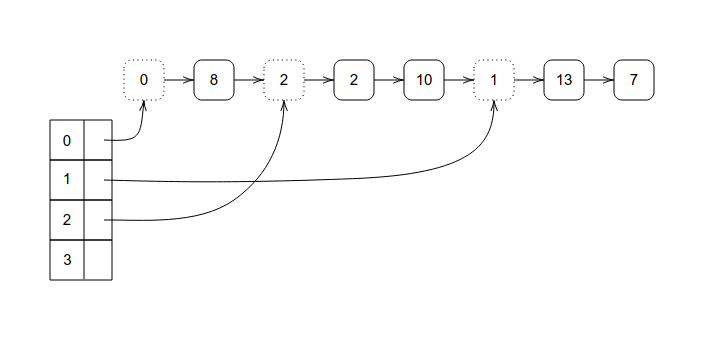
\includegraphics[width=\textwidth]{split-ordered-list-diagram.png}
\caption{The layout of the split-ordered list}
\label{fig:split-order}
\end{figure}

\begin{figure}
    \centering
    \subfloat[Initial state]{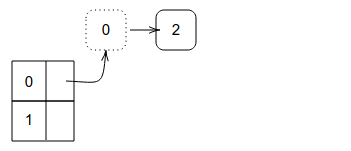
\includegraphics[width=.5\textwidth]{insert-0.png}}
    \subfloat[Dummy node is created]{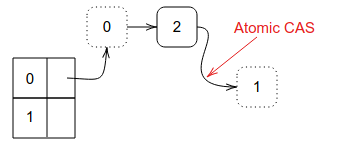
\includegraphics[width=.5\textwidth]{insert-1.png}}
    \newline
    \subfloat[Dummy node is inserted in bucket]{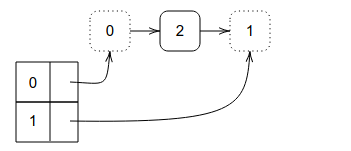
\includegraphics[width=.5\textwidth]{insert-2.png}}
    \subfloat[New node is inserted]{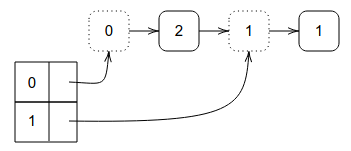
\includegraphics[width=.5\textwidth]{insert-3.png}}
\caption{Insertion without bucket splitting}    
\label{fig:simple-insert}
\end{figure}

\begin{figure}
    \centering
    \subfloat[Initial state]{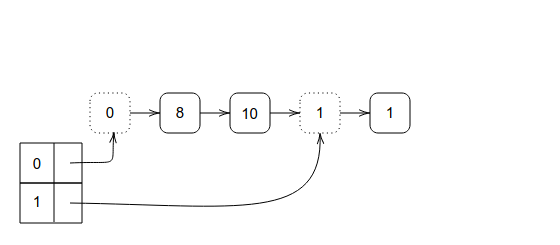
\includegraphics[height=2in]{expand-0.png}}
    \newline
    \subfloat[Table is expanded]{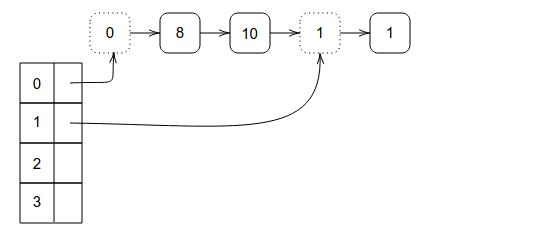
\includegraphics[height=2in]{expand-1.png}}
    \newline
    \subfloat[Dummy node for new bucket inserted]{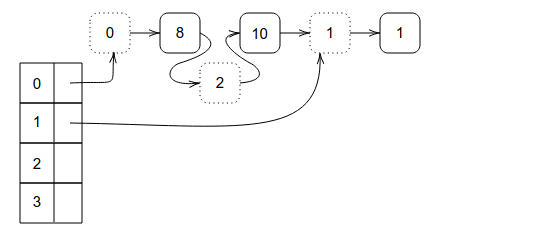
\includegraphics[height=2in]{expand-2.png}}
    \newline
    \subfloat[Table entry points to bucket node]{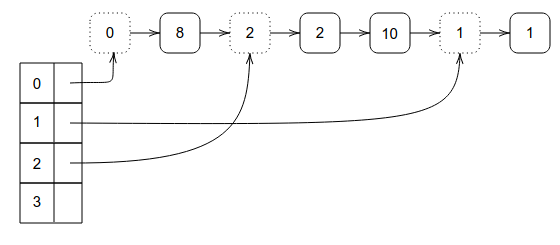
\includegraphics[height=2in]{expand-3.png}}
\caption{Expansion and bucket splitting}    
\label{fig:insert-expand}
\end{figure}


\chapter{Specification}\label{ch:specification}
%intro
% structure of this chapter, structure of the spec, scope
This chapter describes the structure of the TLA+ specification and the process of writing the specification. First we introduce the goals and scope of the specification, then describe the definitions of necessary data structures and operations.
\\\\
The specification consists of two main parts:
\begin{enumerate}
    \item a generic hashmap and
    \item an [insert name of structure here] \textit{implementing} this map.
\end{enumerate}
The generic specification describes the workings of a hashmap with insert and remove operations and ensures that this structure behaves as specified. The [insert name of structure] specification describes Shalev et al.'s specific structure and algorithms for implementing hashmap functionality.
\\\\
We present two versions of the specification at two levels of granularity. The first assumes the atomicity of hashmap operations, while the second describes entirely concurrent operations.

\section{Goal}\label{sec:spec-goals}
The purpose of our specification is to verify the claims about correctness made by Shalev et al. Because TLA+ is designed for checking liveness and safety properties~\cite{Lund2019} we will not check claims about the performance of the implementation. This leaves 4 invariants:
\begin{itemize}
    \item the list beginning at bucket 0 is always sorted
    \item if a bucket is initialized, then it points to a dummy node which is in the list beginning at bucket 0
    \item if a key $k$ is in the map, then \texttt{insert(k)} fails. Otherwise $k$ is added to the map
    \item if a key $k$ is in the map, then \texttt{remove(k)} removes it from the map. Otherwise it fails.
\end{itemize}
The non-concurrent specification demonstrates correctness by implementing a generic hashmap specification which describes corerct behavior, while the concurrent specification looks directly at the above invariants.
Additionally we will check \textit{type safety}: at every point of execution, all keys and values are members of predefined key- and value-sets, respectively.

\section{Non-Concurrent Specification}
\subsection{Hashmap for Implementation}
\begin{figure}
    \begin{tla}
        ------------------------------ MODULE hashmap ------------------------------
(*****************************************************************************)
(*This module describes a hashmap to be used for testing with Shalev et al.'s*)
(*split-ordered list implementation of the data structure                    *)
(*****************************************************************************)

EXTENDS Integers

CONSTANTS NULL, PossibleKeys, PossibleValues

VARIABLES keys, map


(*******************************************************)
(*Initial state has empty map and no keys              *)
(*******************************************************)

HashmapInit ==  /\ keys = {}
                /\ map = [k \in PossibleKeys |-> NULL]

(*******************************************************)
(*Insert changes exactly one mapping of the hashmap    *)
(*and adds one key to the set of keys                  *)
(*******************************************************)
Insert ==   \exists k \in PossibleKeys :
                \exists v \in PossibleValues :
                    /\ keys' = keys \union {k}
                    /\ map' = [map EXCEPT ![k] = v]

(*******************************************************)
(*Remove sets exactly one mapping to NULL              *)
(*******************************************************)
Remove ==   \exists k \in PossibleKeys :
                /\ keys' = keys \ {k}
                /\ map' = [map EXCEPT ![k] = NULL]

(*******************************************************)
(*Next is either an insert, a remove or a find         *)
(*Find(k) returns NULL if not in map, otherwise a value*)
(*******************************************************)          
HashmapNext ==  \/ Insert
                \/ Remove


(*******************************************************)
(*TypeOK asserts all keys and values are of the right type*)
(*******************************************************) 
TypeOK ==   \forall k \in keys :
                /\ k \in PossibleKeys
                /\ map[k] \in PossibleValues

(*******************************************************)
(*KeyHasValue asserts that every key is mapped to a value*)
(*******************************************************) 
KeyHasValue == \forall k \in keys : ~(map[k] = NULL)

(*******************************************************)
(*The hashmap specification as a temporal formula      *)
(*******************************************************) 
HashmapSpec == HashmapInit /\ [][HashmapNext]_<<keys, map>>
=============================================================================
    \end{tla}
\begin{tlatex}
\@x{\@s{32.8}}\moduleLeftDash\@xx{ {\MODULE} hashmap}\moduleRightDash\@xx{}%
\begin{lcom}{0}%
\begin{cpar}{0}{F}{F}{0}{0}{}%
This module describes a hashmap to be used for testing with Shalev et al.'s
 split-ordered list implementation of the data structure                    
\end{cpar}%
\end{lcom}%
\@pvspace{8.0pt}%
\@x{ {\EXTENDS} Integers}%
\@pvspace{8.0pt}%
\@x{ {\CONSTANTS} NULL ,\, PossibleKeys ,\, PossibleValues}%
\@pvspace{8.0pt}%
\@x{ {\VARIABLES} keys ,\, map}%
\@pvspace{16.0pt}%
\begin{lcom}{0}%
\begin{cpar}{0}{F}{F}{0}{0}{}%
Initial state has empty map and no keys              
\end{cpar}%
\end{lcom}%
\@pvspace{8.0pt}%
\@x{ HashmapInit \.{\defeq}\@s{4.1} \.{\land} keys \.{=} \{ \}}%
\@x{\@s{4.1} \.{\land} map \.{=} [ k \.{\in} PossibleKeys \.{\mapsto} NULL ]}%
\@pvspace{8.0pt}%
\begin{lcom}{0}%
\begin{cpar}{0}{F}{F}{0}{0}{}%
Insert changes exactly one mapping of the hashmap    
 and adds one key to the set of keys                  
\end{cpar}%
\end{lcom}%
\@x{ Insert \.{\defeq}\@s{8.2} \exists\, k \.{\in} PossibleKeys \.{:}}%
\@x{\@s{24.59} \exists\, v \.{\in} PossibleValues \.{:}}%
\@x{\@s{41.0} \.{\land} keys \.{'} \.{=} keys \.{\cup} \{ k \}}%
 \@x{\@s{41.0} \.{\land} map \.{'} \.{=} [ map {\EXCEPT} {\bang} [ k ] \.{=} v
 ]}%
\@pvspace{8.0pt}%
\begin{lcom}{0}%
\begin{cpar}{0}{F}{F}{0}{0}{}%
Remove sets exactly one mapping to NULL              
\end{cpar}%
\end{lcom}%
\@x{ Remove \.{\defeq}\@s{8.2} \exists\, k \.{\in} PossibleKeys \.{:}}%
\@x{\@s{24.59} \.{\land} keys \.{'} \.{=} keys \.{\,\backslash\,} \{ k \}}%
 \@x{\@s{24.59} \.{\land} map \.{'} \.{=} [ map {\EXCEPT} {\bang} [ k ] \.{=}
 NULL ]}%
\@pvspace{8.0pt}%
\begin{lcom}{0}%
\begin{cpar}{0}{F}{F}{0}{0}{}%
Next is either an insert, a remove or a find         
 Find(k) returns NULL if not in map, otherwise a value
\end{cpar}%
\end{lcom}%
\@x{ HashmapNext \.{\defeq}\@s{4.1} \.{\lor} Insert}%
\@x{\@s{4.1} \.{\lor} Remove}%
\@pvspace{16.0pt}%
\begin{lcom}{0}%
\begin{cpar}{0}{F}{F}{0}{0}{}%
TypeOK asserts all keys and values are of the right type
\end{cpar}%
\end{lcom}%
\@x{ TypeOK \.{\defeq}\@s{8.2} \forall\, k \.{\in} keys \.{:}}%
\@x{\@s{24.59} \.{\land} k \.{\in} PossibleKeys}%
\@x{\@s{24.59} \.{\land} map [ k ] \.{\in} PossibleValues}%
\@pvspace{8.0pt}%
\begin{lcom}{0}%
\begin{cpar}{0}{F}{F}{0}{0}{}%
KeyHasValue asserts that every key is mapped to a value
\end{cpar}%
\end{lcom}%
 \@x{ KeyHasValue \.{\defeq} \forall\, k \.{\in} keys \.{:} {\lnot} ( map [ k
 ] \.{=} NULL )}%
\@pvspace{8.0pt}%
\begin{lcom}{0}%
\begin{cpar}{0}{F}{F}{0}{0}{}%
The hashmap specification as a temporal formula      
\end{cpar}%
\end{lcom}%
 \@x{ HashmapSpec \.{\defeq} HashmapInit \.{\land} {\Box} [ HashmapNext ]_{
 {\langle} keys ,\, map {\rangle}}}%
\@x{}\bottombar\@xx{}%
\end{tlatex}
    \caption{The hashmap specification}
    \label{fig:hashmap-spec}
\end{figure}
The generic hashmap specification seen in \autoref{fig:hashmap-spec} describes how a hashmap \textit{should} behave. It maintains a set of keys \textit{keys} and a mapping \textit{map} from keys to values. Additionally it describes two operations: insert and remove.
\\\\
Insert adds a key to the set of keys and changes one entry in the map. The key is added with a set union, which preserves key uniqueness. Updating the map uses the \texttt{EXCEPT} construct, to say "the map is the same except the new key maps to the new value". The insert action is always enabled since there will always be keys and values in PossibleKeys and PossibleValues.
\\\\
Remove removes one key from the set and changes its mapping to NULL. This is done through the set difference operator and the same \texttt{EXCEPT} construct as in insert. Both operations are idempotent, so attempting to remove a key that is not in the map will result in no change.
\\\\
The specification also contains temporal formulae \textit{TypeOK} and \textit{KeyHasValue} that specify correct behavior. These have been checked with the TLC model checker [insert results here maybe?].
\\\\
Finally the entire hashmap is described by \textit{HashmapSpec}. This temporal formula states that the hashmap specification is fulfilled if the initial state fulfills \textit{HashmapInit} and each action fulfills \textit{HashmapNext}. This formula is used to prove a more complex specification implements the semantics of Hashmap.
\\\\
The theorem $SOSpec \Rightarrow HashmapSpec$ states that any program following the split-order specification also follows the hashmap specification. Hence, any program following the split-order specification is a correct implementation of a hashmap. It is tested by checking the property \textit{HashmapSpec} in a model checking SOSpec.

\subsection{Non-Concurrent Specification}\label{subsec:non-concurrent}
The specification consists of three main parts:
\begin{enumerate}
    \item \label{SpecList:structures} the data structures,
    \item \label{SpecList:operations} operations on the map, and
    \item \label{SpecList:spec} the abstract specification tying them together.
\end{enumerate}
This section describes the construction and function of each in turn.
\begin{figure}
    \begin{tla}
EXTENDS Integers

CONSTANTS NULL, PossibleKeys, PossibleValues, LoadFactor, MaxSize

VARIABLES keys, AuxKeys, list, buckets, size, count, map

ASSUME
    /\ PossibleKeys \subseteq 0..15
    /\ NULL \notin PossibleKeys
    /\ NULL \notin PossibleValues

(****************************************************)
(*The Init for split-order                          *)
(*keys is initially empty                           *)
(*the map maps every possible key to NULL           *)
(*The list initially contains only the 0 dummy node *)
(****************************************************)
SOInit ==   /\ keys = {}
            /\ AuxKeys = {}
            /\ list = [n \in 0..255 |-> IF n = 0 THEN SODummyKey(0) ELSE NULL]
            /\ buckets = [m \in PossibleKeys |-> IF m = 0 THEN SODummyKey(0) ELSE NULL]
            /\ size = 1
            /\ count = 0
            /\ map = [k \in PossibleKeys |-> NULL]

\end{tla}
\begin{tlatex}
\@x{ {\EXTENDS} Integers}%
\@pvspace{8.0pt}%
 \@x{ {\CONSTANTS} NULL ,\, PossibleKeys ,\, PossibleValues ,\, LoadFactor ,\,
 MaxSize}%
\@pvspace{8.0pt}%
 \@x{ {\VARIABLES} keys ,\, AuxKeys ,\, list ,\, buckets ,\, size ,\, count
 ,\, map}%
\@pvspace{8.0pt}%
\@x{ {\ASSUME}}%
\@x{\@s{16.4} \.{\land} PossibleKeys \.{\subseteq} 0 \.{\dotdot} 15}%
\@x{\@s{16.4} \.{\land} NULL \.{\notin} PossibleKeys}%
\@x{\@s{16.4} \.{\land} NULL \.{\notin} PossibleValues}%
\@pvspace{8.0pt}%
\begin{lcom}{0}%
\begin{cpar}{0}{F}{F}{0}{0}{}%
The Init for split-order                          
 keys is initially empty                           
 the map maps every possible key to NULL           
 The list initially contains only the 0 dummy node 
\end{cpar}%
\end{lcom}%
\@x{ SOInit \.{\defeq}\@s{8.2} \.{\land} keys \.{=} \{ \}}%
\@x{\@s{8.2} \.{\land} AuxKeys \.{=} \{ \}}%
 \@x{\@s{8.2} \.{\land} list \.{=} [ n \.{\in} 0 \.{\dotdot} 255 \.{\mapsto}
 {\IF} n \.{=} 0 \.{\THEN} SODummyKey ( 0 ) \.{\ELSE} NULL ]}%
 \@x{\@s{8.2} \.{\land} buckets \.{=} [ m \.{\in} PossibleKeys \.{\mapsto}
 {\IF} m \.{=} 0 \.{\THEN} SODummyKey ( 0 ) \.{\ELSE} NULL ]}%
\@x{\@s{8.2} \.{\land} size \.{=} 1}%
\@x{\@s{8.2} \.{\land} count \.{=} 0}%
\@x{\@s{8.2} \.{\land} map \.{=} [ k \.{\in} PossibleKeys \.{\mapsto} NULL ]}%
\@pvspace{8.0pt}%
\end{tlatex}
\caption{The initial state of the specification}
\label{fig:SO-init}
\end{figure}
\\\\
The necessary data structures are a list of nodes and an array of buckets pointing to nodes. These are both specified as TLA+ functions. The list is a function from the set of list-keys to the set of values, while bucekts is a function from keys to list-keys. Additionally the specification includes a set of keys and a map from keys to values that correspond to the keys and map in the generic specification. The initial state of the map, showing these structures and their initial values is shown in \autoref{fig:SO-init}

\begin{figure}
\begin{tla}
SOInsert == /\  \E k \in PossibleKeys :
                \E v \in PossibleValues :
                    BucketInsert(k, v)

BucketInsert(k, v) ==
(*Either a bucket needs to be initialized*)
    \/  /\ buckets[k % size] = NULL
        /\ BucketInit(k % size)
        /\ ListInsert(SORegularKey(k), v)
        /\ AuxKeys' = AuxKeys \union {k}                      
    (*Or the bucket is already initialized*)
    \/  /\ buckets[k % size] /= NULL
        /\ ListInsert(SORegularKey(k), v)
        /\ AuxKeys' = AuxKeys \union {k}
        /\ UNCHANGED <<buckets>>

ListInsert(k, v) == IF list[k] = NULL
                THEN list' = [list EXCEPT ![k] = v] /\ count' = count + 1
                ELSE UNCHANGED <<list, count>>

\end{tla} 
\begin{tlatex}
\@x{ SOInsert \.{\defeq} \.{\land}\@s{4.1} \E\, k \.{\in} PossibleKeys \.{:}}%
\@x{\@s{4.1} \E\, v \.{\in} PossibleValues \.{:}}%
\@x{\@s{8.2} BucketInsert ( k ,\, v )}%
\@pvspace{8.0pt}%
\@x{ BucketInsert ( k ,\, v ) \.{\defeq}}%
\@x{}%
\@y{%
 Either a bucket needs to be initialized
}%
\@xx{}%
 \@x{\@s{16.4} \.{\lor}\@s{4.1} \.{\land} buckets [ k \.{\%} size ] \.{=}
 NULL}%
\@x{\@s{20.5} \.{\land} BucketInit ( k \.{\%} size )}%
\@x{\@s{20.5} \.{\land} ListInsert ( SORegularKey ( k ) ,\, v )}%
\@x{\@s{20.5} \.{\land} AuxKeys \.{'} \.{=} AuxKeys \.{\cup} \{ k \}}%
\@x{\@s{16.4}}%
\@y{%
 Or the bucket is already initialized
}%
\@xx{}%
 \@x{\@s{16.4} \.{\lor}\@s{4.1} \.{\land} buckets [ k \.{\%} size ] \.{\neq}
 NULL}%
\@x{\@s{20.5} \.{\land} ListInsert ( SORegularKey ( k ) ,\, v )}%
\@x{\@s{20.5} \.{\land} AuxKeys \.{'} \.{=} AuxKeys \.{\cup} \{ k \}}%
\@x{\@s{20.5} \.{\land} {\UNCHANGED} {\langle} buckets {\rangle}}%
\@pvspace{8.0pt}%
\@x{ ListInsert ( k ,\, v ) \.{\defeq} {\IF} list [ k ] \.{=} NULL}%
 \@x{\@s{4.1} \.{\THEN} list \.{'} \.{=} [ list {\EXCEPT} {\bang} [ k ] \.{=}
 v ] \.{\land} count \.{'} \.{=} count \.{+} 1}%
\@x{\@s{4.1} \.{\ELSE} {\UNCHANGED} {\langle} list ,\, count {\rangle}}%
\@pvspace{8.0pt}%
\end{tlatex}
\caption{The \textit{Insert} operation}
\label{fig:SO-insert}
\end{figure}
\\\\
The \textit{Insert} and \textit{Remove} operations are written in three layers. \autoref{fig:SO-insert} shows the Insert operation. First, \textit{SOInsert} describes a very high-level view: there exists some key and some value, and we insert the value with that key. \textit{BucketInsert} is the most involved, corresponding to the insert operation described by Shalev et al.'s pseudocode~\cite{Shalev2006}. Here the correct bucket is found or initialized and the value is inserted into the list pointed to by this bucket with the split-order key. FInally, \textit{ListInsert} inserts the value into the list, or ignores it if the node already has a value.

\begin{figure}
    \begin{tla}
        SONext ==   \/ SOInsert /\ BucketGrow /\ UNCHANGED <<map, keys>>
            \/ SORemove /\ UNCHANGED <<size, map, keys>>
            \/ SOFind   /\ UNCHANGED <<size, count, list>>
    \end{tla}
\begin{tlatex}
 \@x{\@s{32.8} SONext \.{\defeq}\@s{8.2} \.{\lor} SOInsert \.{\land}
 BucketGrow \.{\land} {\UNCHANGED} {\langle} map ,\, keys {\rangle}}%
 \@x{\@s{49.19} \.{\lor} SORemove \.{\land} {\UNCHANGED} {\langle} size ,\,
 map ,\, keys {\rangle}}%
 \@x{\@s{49.19} \.{\lor} SOFind \.{\land} {\UNCHANGED} {\langle} size ,\,
 count ,\, list {\rangle}}%
\end{tlatex}
    \caption{The Next action}
    \label{fig:SO-next}
\end{figure}
\\\\
Finally, the \textit{Next} action shown in \autoref{fig:SO-next} describes the transition of the system from one state to another. It states that such a transition consists of either inserting and growing the map, removing, or the \textit{SOFind} operation.

\begin{figure}
    \begin{tla}
        SOFind == \E k \in AuxKeys :
                /\ keys' = keys \union {k}
                /\ AuxKeys' = AuxKeys \ {k}
                /\ IF buckets[k % size] = NULL
                     THEN /\ BucketInit(k % size)
                          /\ map' = [map EXCEPT ![k] = ListFind(k % size, SORegularKey(k))]
                     ELSE /\ UNCHANGED buckets
                          /\ map' = [map EXCEPT ![k] = ListFind(k % size, SORegularKey(k))]

    \end{tla}
\begin{tlatex}
\@x{\@s{32.8} SOFind \.{\defeq} \E\, k \.{\in} AuxKeys \.{:}}%
\@x{\@s{36.89} \.{\land} keys \.{'} \.{=} keys \.{\cup} \{ k \}}%
 \@x{\@s{36.89} \.{\land} AuxKeys \.{'} \.{=} AuxKeys \.{\,\backslash\,} \{ k
 \}}%
\@x{\@s{36.89} \.{\land} {\IF} buckets [ k \.{\%} size ] \.{=} NULL}%
\@x{\@s{45.1} \.{\THEN} \.{\land} BucketInit ( k \.{\%} size )}%
 \@x{\@s{45.1} \.{\land} map \.{'} \.{=} [ map {\EXCEPT} {\bang} [ k ] \.{=}
 ListFind ( k \.{\%} size ,\, SORegularKey ( k ) ) ]}%
\@x{\@s{45.1} \.{\ELSE} \.{\land} {\UNCHANGED} buckets}%
 \@x{\@s{45.1} \.{\land} map \.{'} \.{=} [ map {\EXCEPT} {\bang} [ k ] \.{=}
 ListFind ( k \.{\%} size ,\, SORegularKey ( k ) ) ]}%
\@pvspace{8.0pt}%
\end{tlatex}
    \caption{The \textit{SOFind} operation}
    \label{fig:SO-find}
\end{figure}
\begin{figure}
    \begin{tla}
    SOSpec == SOInit /\ [][SONext]_<<keys, AuxKeys, list, buckets, size, count, map>>

    INSTANCE hashmap

    THEOREM SOSpec => HashmapSpec
    \end{tla}
\begin{tlatex}
 \@x{\@s{16.4} SOSpec \.{\defeq} SOInit \.{\land} {\Box} [ SONext ]_{
 {\langle} keys ,\, AuxKeys ,\, list ,\, buckets ,\, size ,\, count ,\, map
 {\rangle}}}%
\@pvspace{8.0pt}%
\@x{\@s{16.4} {\INSTANCE} hashmap}%
\@pvspace{8.0pt}%
\@x{\@s{16.4} {\THEOREM} SOSpec \.{\implies} HashmapSpec}%
\end{tlatex}
    \caption{Implementation of generic hashmap}
    \label{fig:SO-implementation}
\end{figure}
\\\\
The \textit{SOFind} operation shown in \autoref{fig:SO-find} corresponds to the find operation in Shalev et al.'s pseudocode and is responsible for updating the map. Because we wish to show that this specification implements the generic hashmap it is necessary to update the set of keys and the map itself at the same time and so a set of auxiliary keys is maintained and only added to the "real" map once a find operation looks for them. Using the "working variables" trick, the specification can be shown to implement the generic hashmap through implication as seen in \autoref{fig:SO-implementation}.

\subsection{Concurrent Specification}
\begin{figure}
    \begin{tla}
OperationStates ==
    (*Set of all possible active operations            *)
    (*They can be of type insert, delete or bucket\_init*)
    (*Step denotes the current step of the operation   *)
    [type: {"insert"}, step : 1..4, key : PossibleKeys, value : PossibleValues]
        \union 
    [type: {"delete"}, step : 1..3, key : PossibleKeys]
        \union 
    [type: {"bucket_init"}, step : 1..3, bucket : 0..(MaxSize-1)]
    \end{tla}
\begin{tlatex}
\@x{ OperationStates \.{\defeq}}%
\@x{\@s{16.4}}%
\@y{%
 Set of all possible active operations            
}%
\@xx{}%
\@x{\@s{16.4}}%
\@y{%
 They can be of type insert, delete or bucket\_init
}%
\@xx{}%
\@x{\@s{16.4}}%
\@y{%
 Step denotes the current step of the operation   
}%
\@xx{}%
 \@x{\@s{16.4} [ type \.{:} \{\@w{insert} \} ,\, step \.{:} 1 \.{\dotdot} 4
 ,\, key \.{:} PossibleKeys ,\, value \.{:} PossibleValues ]}%
\@x{\@s{28.69} \.{\cup}}%
 \@x{\@s{16.4} [ type \.{:} \{\@w{delete} \} ,\, step \.{:} 1 \.{\dotdot} 3
 ,\, key \.{:} PossibleKeys ]}%
\@x{\@s{28.69} \.{\cup}}%
 \@x{\@s{16.4} [ type \.{:} \{\@w{bucket\_init} \} ,\, step \.{:} 1
 \.{\dotdot} 3 ,\, bucket \.{:} 0 \.{\dotdot} ( MaxSize \.{-} 1 ) ]}%
\end{tlatex}
    \caption{The operation structures}
    \label{fig:op-structure}
\end{figure}

\begin{figure}
    \begin{tla}
        (*Begin an insert operation*)
        Insert(k, v) == activeOps' = activeOps \union {[type|-> {"insert"}, step |-> 1, key |-> k, value |-> v]}           
        (*Begin a delete operation*)
        Delete(k) == activeOps' = activeOps \union {[type|-> {"delete"}, step |-> 1, key |-> k]}
        (*Begin a bucket\_init operation*)
        BucketInit(b) == activeOps' = activeOps \union {[type|-> {"bucket_init"}, step |-> 1, bucket |-> b]}
        
        NextStep(op) == activeOps' = (activeOps \ {op}) \union {[op EXCEPT !["step"] = op.step + 1]}
        End(op) == activeOps' = activeOps \ {op}
    \end{tla}
\begin{tlatex}
\@x{\@s{32.8}}%
\@y{%
 Begin an insert operation
}%
\@xx{}%
 \@x{\@s{32.8} Insert ( k ,\, v ) \.{\defeq} activeOps \.{'} \.{=} activeOps
 \.{\cup} \{ [ type \.{\mapsto} \{\@w{insert} \} ,\, step \.{\mapsto} 1 ,\,
 key \.{\mapsto} k ,\, value \.{\mapsto} v ] \}}%
\@x{\@s{32.8}}%
\@y{%
 Begin a delete operation
}%
\@xx{}%
 \@x{\@s{32.8} Delete ( k ) \.{\defeq} activeOps \.{'} \.{=} activeOps
 \.{\cup} \{ [ type \.{\mapsto} \{\@w{delete} \} ,\, step \.{\mapsto} 1 ,\,
 key \.{\mapsto} k ] \}}%
\@x{\@s{32.8}}%
\@y{%
 Begin a bucket\_init operation
}%
\@xx{}%
 \@x{\@s{32.8} BucketInit ( b ) \.{\defeq} activeOps \.{'} \.{=} activeOps
 \.{\cup} \{ [ type \.{\mapsto} \{\@w{bucket\_init} \} ,\, step \.{\mapsto} 1
 ,\, bucket \.{\mapsto} b ] \}}%
\@pvspace{8.0pt}%
 \@x{\@s{32.8} NextStep ( op ) \.{\defeq} activeOps \.{'} \.{=} ( activeOps
 \.{\,\backslash\,} \{ op \} ) \.{\cup} \{ [ op {\EXCEPT} {\bang} [\@w{step}
 ] \.{=} op . step \.{+} 1 ] \}}%
 \@x{\@s{32.8} End ( op ) \.{\defeq} activeOps \.{'} \.{=} activeOps
 \.{\,\backslash\,} \{ op \}}%
\end{tlatex}
    \caption{Starting and stepping through operations}
    \label{fig:op-progress}
\end{figure}

\begin{figure}
    \begin{tla}
        SONext ==
        \/  /\ \E k \in PossibleKeys :
                 \E v \in PossibleValues :
                    Insert(k, v)
            /\ UNCHANGED <<buckets, count, list, size>>
        \/  /\ \E k \in PossibleKeys :
                Delete(k)
            /\ UNCHANGED <<buckets, count, list, size>>
        \/ Insert1
        \/ Insert2
        \/ Insert3
        \/ Insert4
        \/ Delete1
        \/ Delete2
        \/ Delete3
        \/ BucketInit1
        \/ BucketInit2
        \/ BucketInit3
    \end{tla}
\begin{tlatex}
\@x{\@s{32.8} SONext \.{\defeq}}%
\@x{\@s{32.8} \.{\lor}\@s{4.1} \.{\land} \E\, k \.{\in} PossibleKeys \.{:}}%
\@x{\@s{45.1} \E\, v \.{\in} PossibleValues \.{:}}%
\@x{\@s{45.1} Insert ( k ,\, v )}%
 \@x{\@s{36.89} \.{\land} {\UNCHANGED} {\langle} buckets ,\, count ,\, list
 ,\, size {\rangle}}%
\@x{\@s{32.8} \.{\lor}\@s{4.09} \.{\land} \E\, k \.{\in} PossibleKeys \.{:}}%
\@x{\@s{40.99} Delete ( k )}%
 \@x{\@s{36.89} \.{\land} {\UNCHANGED} {\langle} buckets ,\, count ,\, list
 ,\, size {\rangle}}%
\@x{\@s{32.8} \.{\lor} Insert1}%
\@x{\@s{32.8} \.{\lor} Insert2}%
\@x{\@s{32.8} \.{\lor} Insert3}%
\@x{\@s{32.8} \.{\lor} Insert4}%
\@x{\@s{32.8} \.{\lor} Delete1}%
\@x{\@s{32.8} \.{\lor} Delete2}%
\@x{\@s{32.8} \.{\lor} Delete3}%
\@x{\@s{32.8} \.{\lor} BucketInit1}%
\@x{\@s{32.8} \.{\lor} BucketInit2}%
\@x{\@s{32.8} \.{\lor} BucketInit3}%
\end{tlatex}
    \caption{The concurrent Next action}
    \label{fig:concurrent-next}
\end{figure}

\begin{figure}
    \begin{tla}
(*Steps of a delete operation*)
Delete1 ==
    (*Start a bucket_init if necessary*)
    \E op \in activeOps :
        /\ op.type = {"delete"}
        /\ op.step = 1
        /\ IF buckets[op.key % size] = NULL
                THEN activeOps' = (activeOps \ {op})
                                    \union {[op EXCEPT !["step"] = op.step + 1]}
                                    \union {[type|-> {"bucket_init"}, step |-> 1, bucket |-> op.key % size]}
                ELSE NextStep(op)
        /\ UNCHANGED <<list, buckets, size, count>>

Delete2 ==
    (*If the key is not there, end operation. Else, remove it*)
    \E op \in activeOps :
        /\ op.type = {"delete"}
        /\ op.step = 2
        /\  IF list[SORegularKey(op.key)] = NULL
                THEN /\ End(op)
                     /\ UNCHANGED list
                ELSE /\ list' = [list EXCEPT ![SORegularKey(op.key)] = NULL]
                     /\ NextStep(op)
        /\ UNCHANGED <<buckets, size, count>>        

Delete3 ==
    (*Decrement count*)
    \E op \in activeOps :
        /\ op.type = {"delete"}
        /\ op.step = 3
        /\ count' = count - 1
        /\ End(op)
        /\ UNCHANGED <<buckets, list, size>>
    \end{tla}
\begin{tlatex}
\@x{}%
\@y{%
 Steps of a delete operation
}%
\@xx{}%
\@x{ Delete1 \.{\defeq}}%
\@x{\@s{16.4}}%
\@y{%
 Start a bucket_init if necessary
}%
\@xx{}%
\@x{\@s{16.4} \E\, op \.{\in} activeOps \.{:}}%
\@x{\@s{20.5} \.{\land} op . type \.{=} \{\@w{delete} \}}%
\@x{\@s{20.5} \.{\land} op . step \.{=} 1}%
\@x{\@s{20.5} \.{\land} {\IF} buckets [ op . key \.{\%} size ] \.{=} NULL}%
 \@x{\@s{28.7} \.{\THEN} activeOps \.{'} \.{=} ( activeOps \.{\,\backslash\,}
 \{ op \} )}%
 \@x{\@s{32.8} \.{\cup} \{ [ op {\EXCEPT} {\bang} [\@w{step} ] \.{=} op . step
 \.{+} 1 ] \}}%
 \@x{\@s{32.8} \.{\cup} \{ [ type \.{\mapsto} \{\@w{bucket\_init} \} ,\, step
 \.{\mapsto} 1 ,\, bucket \.{\mapsto} op . key \.{\%} size ] \}}%
\@x{\@s{28.7} \.{\ELSE} NextStep ( op )}%
 \@x{\@s{20.5} \.{\land} {\UNCHANGED} {\langle} list ,\, buckets ,\, size ,\,
 count {\rangle}}%
\@pvspace{8.0pt}%
\@x{ Delete2 \.{\defeq}}%
\@x{\@s{16.4}}%
\@y{%
 If the key is not there, end operation. Else, remove it
}%
\@xx{}%
\@x{\@s{16.4} \E\, op \.{\in} activeOps \.{:}}%
\@x{\@s{20.5} \.{\land} op . type \.{=} \{\@w{delete} \}}%
\@x{\@s{20.5} \.{\land} op . step \.{=} 2}%
 \@x{\@s{20.5} \.{\land}\@s{4.1} {\IF} list [ SORegularKey ( op . key ) ]
 \.{=} NULL}%
\@x{\@s{28.7} \.{\THEN} \.{\land} End ( op )}%
\@x{\@s{28.7} \.{\land} {\UNCHANGED} list}%
 \@x{\@s{28.7} \.{\ELSE} \.{\land} list \.{'} \.{=} [ list {\EXCEPT} {\bang} [
 SORegularKey ( op . key ) ] \.{=} NULL ]}%
\@x{\@s{28.7} \.{\land} NextStep ( op )}%
 \@x{\@s{20.5} \.{\land} {\UNCHANGED} {\langle} buckets ,\, size ,\, count
 {\rangle}}%
\@pvspace{8.0pt}%
\@x{ Delete3 \.{\defeq}}%
\@x{\@s{16.4}}%
\@y{%
 Decrement count
}%
\@xx{}%
\@x{\@s{16.4} \E\, op \.{\in} activeOps \.{:}}%
\@x{\@s{20.5} \.{\land} op . type \.{=} \{\@w{delete} \}}%
\@x{\@s{20.5} \.{\land} op . step \.{=} 3}%
\@x{\@s{20.5} \.{\land} count \.{'} \.{=} count \.{-} 1}%
\@x{\@s{20.5} \.{\land} End ( op )}%
 \@x{\@s{20.5} \.{\land} {\UNCHANGED} {\langle} buckets ,\, list ,\, size
 {\rangle}}%
\end{tlatex}
    \caption{The steps of a \textit{Delete} operation}
    \label{fig:op-delete}
\end{figure}
The specification described in \autoref{subsec:non-concurrent} describes the working of the split-order structure. However, it is not useful for proving the correctness of the structure in a concurrent setting. This is because its structure presupposes the linearizability of its operations by making them action statements. This means each state transition consists of a complete operation, rather than a single instruction.
\\\\
To specify concurrent working, a more granular specification is needed. In a complete description each step would be a single machine instruction, but this is both infeasible and counterproductive as such a specification is no more useful for verification than the program itself.
\\\\
Instead, we identify the steps in the each operation that change the shared state of the system and make those the steps of our specification. This results in each operation (\textit{Insert, Remove}, and \textit{Bucket Init}) being split into several steps. We then maintain a set of active operations of the form shown in \autoref{fig:op-structure} and step through them as shown in \autoref{fig:op-progress}. The result is the next-step action shown in \autoref{fig:concurrent-next}. This disjunction specifies that each next step can either start an insert or remove operation, or perform a single step in an active operation.
\\\\
To show the structure of a single operation in the concurrent specification, we will look at \textit{Delete} (\autoref{fig:op-delete}). \textit{Delete}1 checks if the relevant bucket is initialized and starts a bucket\_init operation if it is not. Because starting a new operation and advancing the current operation both modify the state of \textit{activeOps}, a union of both changes is needed. Also note that this step is enabled iff there exists an operation with type "delete" and step 1 in the set of active operations. \textit{Delete}2 removes a node from the list. This step is assumed to be atomic by our assumption that an atomic list implementation is available. Finally \textit{Delete}3 decrements count. Note that the previous step did not advance if a node was not removed, so the decrement step will always be taken if a delete operation has reached step 3.

\chapter{Results}\label{ch:results}
\section{Method}
To demonstrate the invariants claimed by Shalev et al.~\cite{Shalev2006} we use the TLC model checker to test the specifications outlined in \autoref{ch:specification}. The first specification (\autoref{subsec:non-concurrent}) was tested by setting the implication
\begin{tla}
    SOSpec => HashmapSpec
\end{tla}
\begin{tlatex}
\@x{\@s{16.4} SOSpec \.{\implies} HashmapSpec}%
\end{tlatex}
as a property of the model, thus showing that SplitOrder implements the generic hashmap specification.
\\\\
\textit{SOConcurrent} is more granular than the abstract specification which makes it difficult to demonstrate an implication. Instead three of the four claimed invariants were written as predicates in TLA (\autoref{fig:invariants}). (The last invariant is the sorted order of the list, which is trivially true due to how the list is represented in TLA.) The first invariant is a claim on each state and can be checked straighforwardly. The remaining two, split into four in TLA, are invariants on behaviors and make use of the temporal operator $\Box$ meaning "always". Additionally, these invariants are written in terms of the constant set of all possible operation states because TLC cannot check liveness properties that include existential quantifiers ($\E$ and $\A$) over variables.
\begin{figure}
    \begin{tla}
(*Each bucket is either unitialized or points to a node with the dummy key*)
BucketsInitialized ==
    \A i \in 0..(size-1) :
        \/ buckets[i] = NULL
        \/ buckets[i] = SODummyKey(i) /\ list[SODummyKey(i)] = i

(*An insert with key not in map will succeed*)
InsertSucceeds ==
    \A op \in OperationStates :
        IF op.type = "insert"
        (*This test is needed to avoid checking fields that do not exist in other types of operations*)
        THEN
            /\ op \in BagToSet(activeOps)
            /\ op.step = 1
            /\ list[SORegularKey(op.key)] = NULL
            => <>(list[SORegularKey(op.key)] = op.value)
        ELSE TRUE

(*A delete with key in map will succeed*)
DeleteSucceeds ==
    \A op \in OperationStates :
        IF op.type = "delete"
        THEN
            /\ op \in BagToSet(activeOps)
            /\ op.step = 1
            /\ list[SORegularKey(op.key)] /= NULL
        => <>(list[SORegularKey(op.key)] = NULL)
        ELSE TRUE
        
    \end{tla}
\begin{tlatex}
\@x{}%
\@y{%
 Each bucket is either unitialized or points to a node with the dummy key
}%
\@xx{}%
\@x{ BucketsInitialized \.{\defeq}}%
\@x{\@s{16.4} \A\, i \.{\in} 0 \.{\dotdot} ( size \.{-} 1 ) \.{:}}%
\@x{\@s{20.5} \.{\lor} buckets [ i ] \.{=} NULL}%
 \@x{\@s{20.5} \.{\lor} buckets [ i ] \.{=} SODummyKey ( i ) \.{\land} list [
 SODummyKey ( i ) ] \.{=} i}%
\@pvspace{8.0pt}%
\@x{}%
\@y{%
 An insert with key not in map will succeed
}%
\@xx{}%
\@x{ InsertSucceeds \.{\defeq}}%
\@x{\@s{16.4} \A\, op \.{\in} OperationStates \.{:}}%
\@x{\@s{20.5} {\IF} op . type \.{=}\@w{insert}}%
\@x{\@s{20.5}}%
\@y{%
 This test is needed to avoid checking fields that do not exist in other
 types of operations
}%
\@xx{}%
\@x{\@s{20.5} \.{\THEN}}%
\@x{\@s{36.9} \.{\land} op \.{\in} BagToSet ( activeOps )}%
\@x{\@s{36.9} \.{\land} op . step \.{=} 1}%
\@x{\@s{36.9} \.{\land} list [ SORegularKey ( op . key ) ] \.{=} NULL}%
 \@x{\@s{36.9} \.{\implies} {\Diamond} ( list [ SORegularKey ( op . key ) ]
 \.{=} op . value )}%
\@x{\@s{20.5} \.{\ELSE} {\TRUE}}%
\@pvspace{8.0pt}%
\@x{}%
\@y{%
 A delete with key in map will succeed
}%
\@xx{}%
\@x{ DeleteSucceeds \.{\defeq}}%
\@x{\@s{16.4} \A\, op \.{\in} OperationStates \.{:}}%
\@x{\@s{20.5} {\IF} op . type \.{=}\@w{delete}}%
\@x{\@s{20.5} \.{\THEN}}%
\@x{\@s{36.9} \.{\land} op \.{\in} BagToSet ( activeOps )}%
\@x{\@s{36.9} \.{\land} op . step \.{=} 1}%
\@x{\@s{36.9} \.{\land} list [ SORegularKey ( op . key ) ] \.{\neq} NULL}%
 \@x{\@s{20.5} \.{\implies} {\Diamond} ( list [ SORegularKey ( op . key ) ]
 \.{=} NULL )}%
\@x{\@s{20.5} \.{\ELSE} {\TRUE}}%
\@pvspace{8.0pt}%
\end{tlatex}
    \caption{The claimed invariants as TLA predicates}
    \label{fig:invariants}
\end{figure}}
\section{Technical Details}
Tests were run with version 2.15 of the TLC model checker on a Intel(R) Core i5-8250U CPU with 8~GiB of memory and 250~GiB of hard drive space running Ubuntu 18.04.
\section{Results}
\subsection{Non-concurrent specification}
[Need to rerun the coarse specification model check (oops)]

\subsection{Concurrent Specification}

\begin{tabular}{ |c|c|c|c||c|c|c| }
    \hline
    Invariant & Keys & Values & Concurrent Ops & Distinct states & Time & Error \\
    \hline
    \textit{InsertSucceeds} & 4 & 2 & 2 & 1,105,192 & 00:02:09 &\\
                            & 4 & 3 & 2 & 902,996   & 00:03:14 & OutOfMemoryError\\

    \hline
\end{tabular}

Lessons learned so far
\begin{itemize}
    \item state space explosion is \textbf{real}
    \item liveness properties tend to quickly exceed Java's GC limit
    \item it's easy to mis-state what you want to check, and to make subtle spec errors if not careful
\end{itemize}

\chapter{Discussion}\label{ch:discussion}
[some sort of introduction]
\\\\
% I learned a lot, but the output does not prove anything about concurrent correctness
% structure of the spec follows the structure of the implementation, which does not lend itself to logical state transitions.
% should have made a more conscious decision about step size
% "correct" thinking: what constitutes the state? when does that change?
% implementation (the proof kind) looked to be elegant, but introduced unwanted complexity
The first attempt at writing a specification served as a learning tool for the TLA+ language, but did not produce a useful specification for the purpose of proving correctness in a concurrent setting. The structure of the specification was based on the structure of an implementation in that actions correspond to the \textit{insert}, \textit{delete} and \textit{bucket init} functions in Shalev et al.'s pseudocode. Such a structure brings with it the implicit assumption that the functions are linearizable since one action corresponds to one state transition.
\\\\
The attempt to show correctness through implementation also posed difficulties. The idealized hashmap specification proved impossible to directly map to the split-order specification because a \textit{find} operation in may result in a bucket needing to be initialized and thus can not be used directly in a refinement mapping. Instead we introduced a set of auxiliary variables~\cite{Lamport2019a} and maintained an idealized map that was updated in atomic steps to implement the Hashmap specification. The updates loosely correspond to a \textit{find} operation and the correctness of this idealized map does seem to correspond to a correct underlying structure (albeit at an earlier state), but introduces additional complexity to the spec and does not resolve the underlying issue of assumed linearizability.
\subsection{Implementation Issues aka. "dumb things I did"}
\backmatter
\printbibliography{}
\appendix
\addcontentsline{toc}{chapter}{Appendix}
% \addtocontents{toc}{\protect\contentsline{chapter}{Appendix:}{}}
\end{document}

